\section{Design and Implementation}
This is a placeholder for an introductory paragraph to our design. Perhaps include a storyboard or something similar to illustrate the basic flow of the application
from the point of view of a user.

\subsection{Key Exchange}
One of the more critical aspects of information security is keeping the private data secret.
The short range of Bluetooth allows for a face-to-face exchange of information that significantly reduces the chances of interception.
Furthermore utilizing the Diffie-Hellman Key Exchange protocol ensures that attackers cannot use intercepted public data to recreate keys.
Lastly Bluetooth's widespread avaliblity in SMS capable devices allowed us to reach a large user base.
This section explains our implementation of these systems.

\subsubsection{Bluetooth Key Generation}
To set up the Bluetooth connection devices must be assigned a server or client role.
Socket controllers are created and managed by a individual threads.
Threading of the connection set up and management is necessary because socket listening and stream reading are blocking statements.
Three threads are managed by a service we have called the Bluetooth service.
A accept thread sets up a server socket to listen for incoming connection requests.
Connect thread sets up the client socket to request connection between this device and the provided device.
Lastly a connected thread manages the input and output streams created when a server and client socket connect.
When a user starts a key exchange the Bluetooth service is created and the accept thread is ran.
The first device to trigger the exchange to begin runs their connect thread.
The two devices connect and both create a BluetoothSocket.
This BluetoothSocket is fed to each device's connected thread.
All remaining threads stop once the connection is established.
What device becomes the client is completely dependent on what user is first to start the exchange.
By setting up each device as a server and making the client role a first come first serve role; the entire connection is seamless to the user.
Figure \ref{fig:serverClient} visualizes this set up.

\begin{figure}
  \includegraphics[width=\linewidth]{serverClient.eps}
  \caption{Bluetooth connection creation.}
  \label{fig:serverClient}
\end{figure}

Once a Bluetooth connection is established a Diffie-Hellman key exchange begins.
\ref{fig:keyExchange} represents this exchange.
Both the server and client send their key expiration ranges to each other.
Expiration ranges are set previously in the app settings.
This range represents the acceptable amount of messages that a key may be used on before it is deleted and the next key is used.
Both devices use the minimum amount agreeable to both users.
If the users settings don't over lap the user with the more secure range will be allowed to select a new expiration count.
The more secure range is defined as the range that has the lowest uses per key.
The more secure use is allowed to chose a expiration count ranging from their maximum to the other users minimum.
This design decision was based on the idea that more secure users should never be punished by being forced to use anything above their maximum setting.

After the parameters are agreed upon the server creates a Java KeyPairGenerator.
KeyPairGenerators created for Diffie-Hellman will result in two keys.
Java uses some confusing terminology with Diffie-Hellman keys.
Java labels secret values, a and b, as private keys and mod values as public keys.
Public keys also contain the p and g parameters used to generate the keys.

The server will generate one hundred public - private keys.
Then encode all public keys and send them over the bluetooth socket to the client.
After receiving the public key values the client will generate its own KeyPairGenerator based on the parameters received from the server.
The client will use the generator to create its own one hundred public - private keys.
In the same matter as before it will package its public keys and send them to the server.
Now that both the server and the client have each others public keys and their private keys one hundred session keys are generated.
The session keys along with the initialization factors and agreed upon key expiration are stored into the contact database.

\begin{figure}
  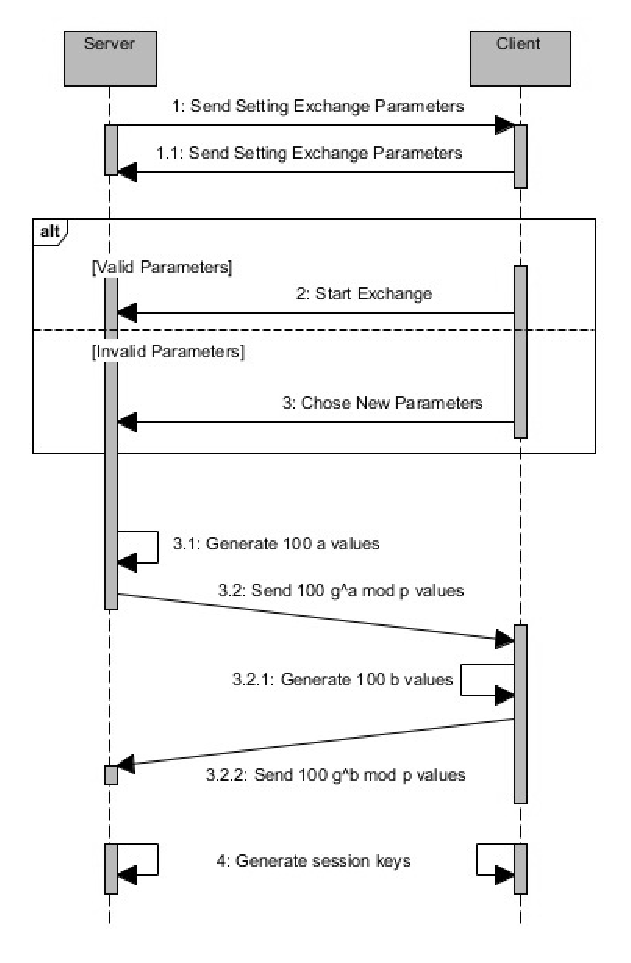
\includegraphics[width=\linewidth]{keyExchange.eps}
  \caption{Diffie-Hellman key exchange.}
  \label{fig:keyExchange}
\end{figure}

\subsubsection{Key Specifics}
The keys are Diffie-Hellman key exchange generated 32-byte secret numbers that are shared between
the two devices. Our application uses the bytes of this 32-byte number as the key for our block cipher.

The cipher implemented is an AES-256 cipher in CBC mode. This cipher handles encryption and
decryption of the text messages. The initialization vector is a randomly generated 128-bit block that
is shared over Bluetooth alongside the keys during exchange.

\subsection{Information Storage and Control}
This is a placeholder for a short paragraph or two that provides an overview of our Information Storage and Control systems.

\subsubsection{BSecure Databases}
To organize key usage to be synchronized between both devices we utilized sequence numbers.
These sequence numbers were sequential integer values associated with each key that represented the
order in which the key would be used. The next key to be used would be determined by incrementing the sequence
number of the previous key.

Explain the sequence number idea (Consumer/Producer control scheme for storage)

Explain key expiration (Each time key is ``used,'' a value is decremented)

Explain how we use the Android Contact\_ID (The primary key of the Android contact DB)

We stored all our important values for maintaining each BSecure associated contact
into a database. The values stored in this database table are used to decide what key to use for that
contact.

Refer to Table \ref{table:contacttable} for the row layout of our SQL database.

\begin{table*}
\centering
\caption{Key Table Design}
\label{table:contacttable}
\begin{tabular}{|c|c|c|c|} \hline
CONTACT\_ID&CURRENT\_SEQUENCE\_NUM&KEY&IV\\ \hline\end{tabular}
\end{table*}

\begin{table*}
\centering
\caption{Contact Table Design}
\label{table:contacttable}
\begin{tabular}{|c|c|c|c|c|c|} \hline
CONTACT\_ID&CURRENT\_SEQUENCE\_NUM&MAX\_SEQUENCE\_NUM&TOTAL\_KEYS&USES\_LEFT&USES\_MAX\\ \hline\end{tabular}
\end{table*}


\subsubsection{User Settings}
Elaborate on settings available to the user

Option to force a current key for a contact to expire

Option to force all keys with a contact to expire

Option to force all keys to expire with all contacts

If the user lacks keys with a contact they can still send unencrypted messages

User chooses a maximum and minimum number of times a key is to be used. During Bluetooth exchange
these values are sent to the other device and a decision is made on which mutual value to use for the maximum key use setting.

\subsection{Use of Text Message Headers}
This is a placeholder for an introductory paragraph on using headers in our text messages.

\subsubsection{BSecure Message Header}
Explain the use of a header in the text message to indicate that the message is from a BSecure application

We appended a header to the beginning of encrypted text messages to flag to the receiving application that
the incomming message is a BSecure encrypted message.

\subsubsection{Expire Current Key Header}
Explain the use of a header to notify that the contact has expired their key early (So keys remain synchronized across both devices).

\subsubsection{Expire All Keys Header}
Explain the use of a header to notify that the contact has expired ALL keys early.


